\documentclass[english]{article}\usepackage[]{graphicx}\usepackage[]{color}
\usepackage{alltt}
\usepackage[T1]{fontenc}
\usepackage[latin9]{inputenc}
\usepackage{geometry}
\geometry{verbose}
\setcounter{secnumdepth}{2}
\setcounter{tocdepth}{2}
\usepackage{amsmath}
\usepackage{graphicx}
\usepackage{esint}
\usepackage{babel}
\usepackage{verbatim} % for \begin{comment}
\usepackage{subcaption}
\IfFileExists{upquote.sty}{\usepackage{upquote}}{}
\begin{document}

\title{Autonomous Robots and Environmental Mapping}

\author{M. Horning, M. Lin, S. Srinivasan, S. Zou}

\maketitle

\begin{abstract}

Compressed sensing is a technique used to reconstruct sparse signals and images while sampling well below the Nyquist rate. Commonly used in fMRIs and medical imaging, we aim to use this technique to allow autonomous robots to map piecewise constant areas of interest within a larger environment. In our experiment, we programmed a robot equipped with a reflectance sensor to travel along straight-line paths on a black testbed with white regions of interest. The robot integrated sensor readings and sent that sum to a remote server after each path. Each data point consists of the robot's start and end positions, tracked by an overhead camera, and the integral found along that path. Once all the data has been collected, the environment is reconstructed by minimizing the sum of the data fitting term and an L1 penalty term. When using an adaptive path selection scheme, preliminary simulations of our experiment show reconstruction of 100x100 images with only 100 data points (relative err. = 0.28), and we have begun trials with data collected by the robot.

\end{abstract}

\pagebreak
\tableofcontents
\pagebreak

\section{Introduction}

\begin{comment}
Discuss Compressed Sensing
\end{comment}



Compressed sensing describes a technique in which a signal is reconstructed by solving an underdetermined linear system. Doing so allows a signal to be found from a relatively small amount of data. 

%%%%%%%%%%%%%%%%%%%%%%%%%%%%%%%%%%%% LAB SETUP %%%%%%%%%%%%%%%%%%%%%%%%%%%%%%%%%%%%%%%%%%%%%%%%%%%
\section{Lab Setup}
\subsection{Testbed}
The setup in the UCLA Applied Mathematics Laboratory (AML) used three main components: an overhead camera with a tracking system, a PC computer, and the robot vehicle. The testbed is a 1.5 m x 2.0 m rectangular area made of black asphalt felt paper. The cars' positions are tracked by 2 overhead Imaging Source DMK 21F04 1/4 Monochrome CCD cameras with a resolution of 640 x 480 pixels. They have a frame rate of 30 fps and are connected to an image processing PC via firewire cable. The cars are identified using an OpenCV contour searching function that recognizes black and white ID tags, or "hats", that are fixed on top of the vehicle, giving the robot's current position and orientation \cite{gonzalez2011third}

This information is then broadcast through a serial radio module to be received by the cars on the testbed, for use in control algorithms. This mimics the functionality of a GPS unit that may be present in more advanced vehicles in the field.
The cars are given commands and can relay status information by communicating via a separate serial radio with an interface PC that serves primarily as a remote terminal for the cars. The ability to broadcast messages to the interface PC for display proves to be a very useful debugging tool.
\subsection{Robot}
\subsection{Video Camera}
\subsection{Server}
\subsection{Putting it all together}
\begin{comment}
Description of testbed, hardware, software, logic
Sid's flowchart
\end{comment}
%%%%%%%%%%%%%%%%%%%%%%%%%%%%%%%%%%%%%%%%%%%%%%%%%%%%%%%%%%%%%%%%%%%%%%%%%%%%%%%%%%%%%%%%%%%%%%%%%%

\section{Models and assumptions}
Our model and lab setup were designed with certain constraints in mind. The model is designed for robots with limited on board storage and computing power. 

\begin{comment}
Description of constraints for our problem
limited bandwidth, data storage
Also assumptions about simple piecewise environments
\end{comment}

\section{Algorithm for solving the inverse problem}
\begin{comment}
\end{comment}
\subsection{Simulated Results}
\label{sec:simresults}
\subsection{Experimental Results}

\section{Comparison with Other Approaches}
\begin{comment}
\end{comment}

In order to judge the effectiveness of our approach, we examine other methods of collecting data and reconstructing an image. Perhaps the most intuitive manner in which to gather data about the image is to sample individual points rather than travelling and integrating along a path. As when collecting data in the form of path integrals, we would want the number of sampled points to be as low as possible. Having sampled points for data, there are then multiple approaches to recovering the image. One approach is to simply use the same Split Bregman iteration that we are using for reconstruction from path integrals, but with the individually sampled pixels. Alternatively, we can take the value found at each pixel and assign the same value to nearby pixels, a method that we refer to as pixel expansion.

Figures \ref{fig:samplerec} and \ref{fig:sampleexp} present reconstructions of the previously shown 50x50 test image using these approaches, both with randomly sampled points and points sampled on a grid. In all cases, 100 pixels are sampled, and the sampled points are colored white.

In Figure \ref{fig:samplerec}, Split Bregman iteration was used with the collected data for reconstruction. The algorithm itself is unchanged, but the equation corresponding to a data point will simply give the value of a pixel rather than weighting pixels along the path. This method provides a moderately good reconstruction, especially in determining the general shape of the region of interest in the environment, but the demarcation between the shades of gray in the image is difficult to distinguish, making the image seem very blurry. This is not surprising because by sampling pixels, the only information gathered is about those specific pixels, so the space in between can gradate as quickly or slowly as the reconstruction algorithm deems fit. By comparing \ref{fig:randrec} and \ref{fig:gridrec}, it appears that the reconstruction is more accurate when the points are 

Figure \ref{fig:sampleexp} illustrates pixel expansion. This is done by looping through every pixel in the image, and for each pixel, finding and assigning the value from the nearest pixel that was sampled.

\begin{figure}
\centering
\begin{subfigure}{.5\textwidth}
  \centering
    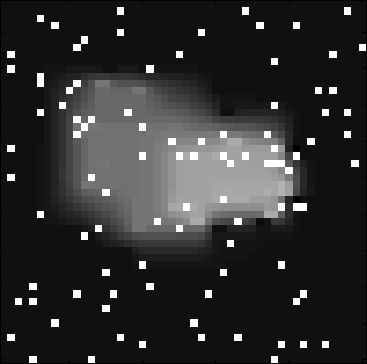
\includegraphics[width=.9\linewidth]{figures/randompointreconstruction}
  \caption{Reconstruction using points sampled randomly.}
  \label{fig:randrec}
\end{subfigure}%
\begin{subfigure}{.5\textwidth}
  \centering
    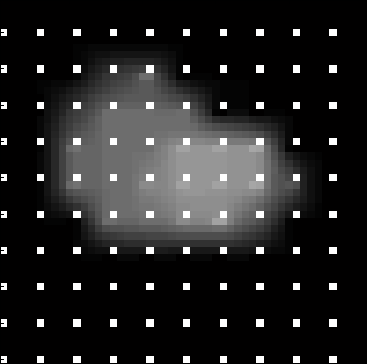
\includegraphics[width=.9\linewidth]{figures/gridpointreconstruction}
  \caption{Reconstruction using points sampled on a grid.}
  \label{fig:gridrec}
\end{subfigure}
\caption{Values are found at sampled points, and Split Bregman iteration is used to reconstruct the image.}
\label{fig:samplerec}
\end{figure}

\begin{figure}
\centering
\begin{subfigure}{.5\textwidth}
  \centering
    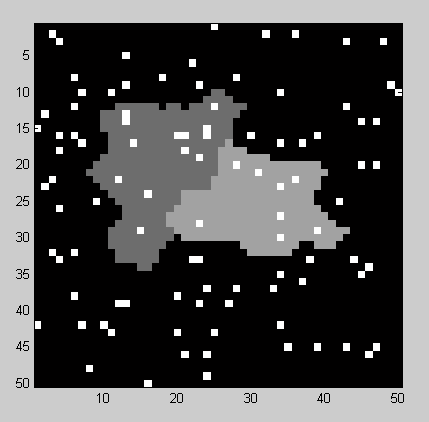
\includegraphics[width=.9\linewidth]{figures/randompointexpansion}
  \caption{Expansion of points sampled randomly.}
  \label{fig:randexp}
\end{subfigure}%
\begin{subfigure}{.5\textwidth}
  \centering
    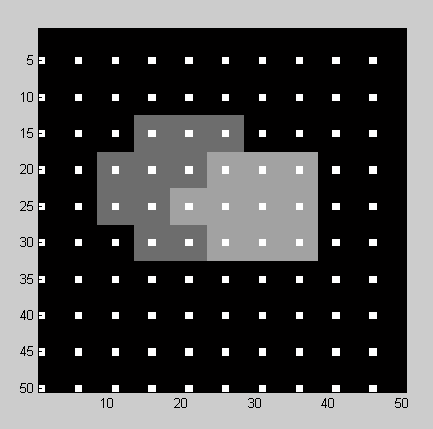
\includegraphics[width=.9\linewidth]{figures/gridpointexpansion}
  \caption{Expansion of points sampled on a grid.}
  \label{fig:gridexp}
\end{subfigure}
\caption{Values are found at sampled points, and those values fill the area surrounding the sampled points.}
\label{fig:sampleexp}
\end{figure}

\begin{figure}
  \centering
    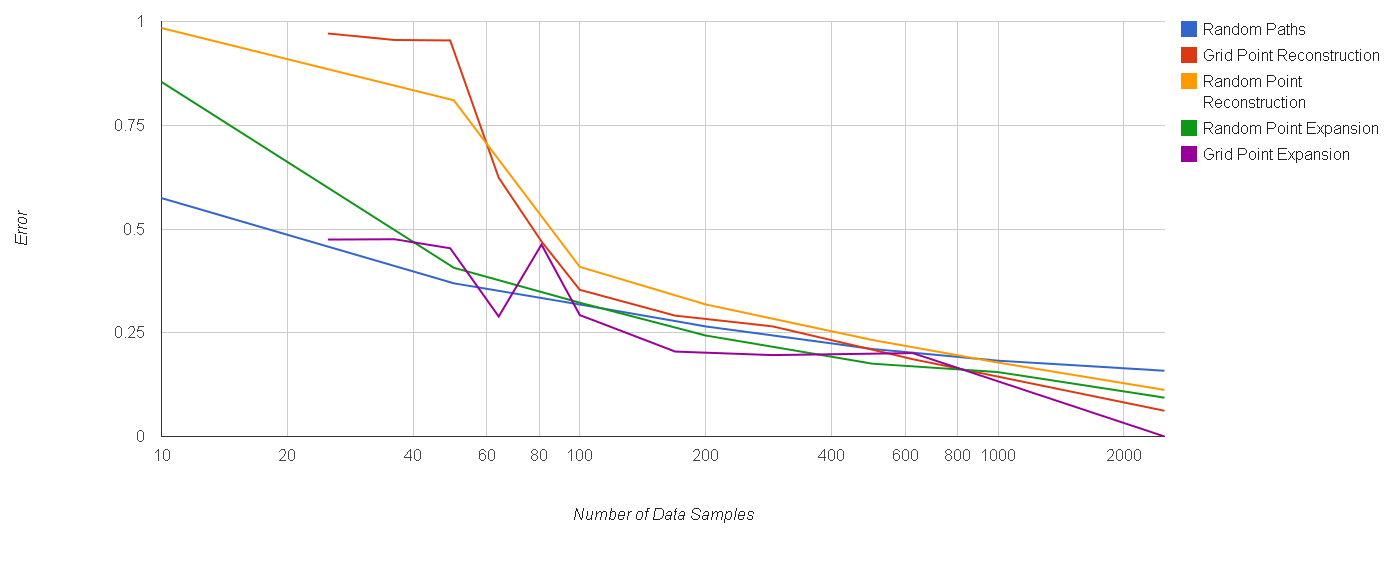
\includegraphics[width=1\textwidth]{figures/othermethoderror}
  \caption{Plot of errors using various reconstruction methods with respect to the number of data samples used.}
  \label{fig:othermethoderror}
\end{figure}

\section{Adaptive Pathing}
\begin{comment}
\end{comment}
\subsection{Simulated Results}
\subsection{Experimental Results}

\section{Conclusions and Further Work}

\newpage
\bibliographystyle{plain}
\bibliography{resources.bib}

\end{document}
